\documentclass[handout]{beamer}
\usepackage[T1]{fontenc}
\usepackage[utf8]{inputenc}
\usepackage{lmodern}
\usepackage[italian]{babel}
\usepackage{mathrsfs}
\usepackage{cancel}
\usepackage{multicol}

\title{I numeri: naturali, interi, decimali}
\author{Mattia Cozzi}
\date{a.f.~2024/2025}
%\documentclass[handout]{beamer}     %usare questa classe per generare l'handout
%\usepackage{pgfpages}   %per mostrare più quadri nella stessa pagina
%\pgfpagesuselayout{4 on 1}[a4paper,border shrink=5mm,landscape]
\usetheme{Singapore}
%\useoutertheme[left]{sidebar} %elementi intorno alle diapositive
\setbeamercovered{dynamic} %modifica l'aspetto del testo grigetto delle diapositive future. Argomenti: invisible/transparent/dynamic

\usecolortheme{orchid}





\theoremstyle{plain}
\newtheorem{teorema}{Teorema}

\usepackage{tikz}
\usepackage{circuitikz}

\usepackage{pgf,pgfplots,graphicx}
\usetikzlibrary{angles,quotes,arrows,shapes,decorations.markings}
\pgfplotsset{compat=1.15}
\usepgfplotslibrary{units,fillbetween} % to add units easily to axis


\def\angolo[#1](#2)(#3:#4:#5)% Syntax: [draw options] (center) (initial angle:final angle:radius)
    { \draw[#1] ($(#2)+({#5*cos(#3)},{#5*sin(#3)})$) arc (#3:#4:#5); }


\begin{document}

\begin{frame}
  \titlepage
\end{frame}





\begin{frame}
\frametitle{Contenuti}
\tableofcontents
\end{frame}


\section{Numeri naturali}


\begin{frame}
\frametitle{Numeri naturali}
I numeri naturali sono i numeri più semplici e i primi che si imparano.\pause

~

\alert{I numeri naturali vengono utilizzati per contare} in generale, ad esempio per indicare quante foglie ha una pianta o quante caramelle ci sono in un vaso.

~

\visible<2->{\begin{columns}
  \begin{column}{0.4\textwidth}
  \begin{figure}
    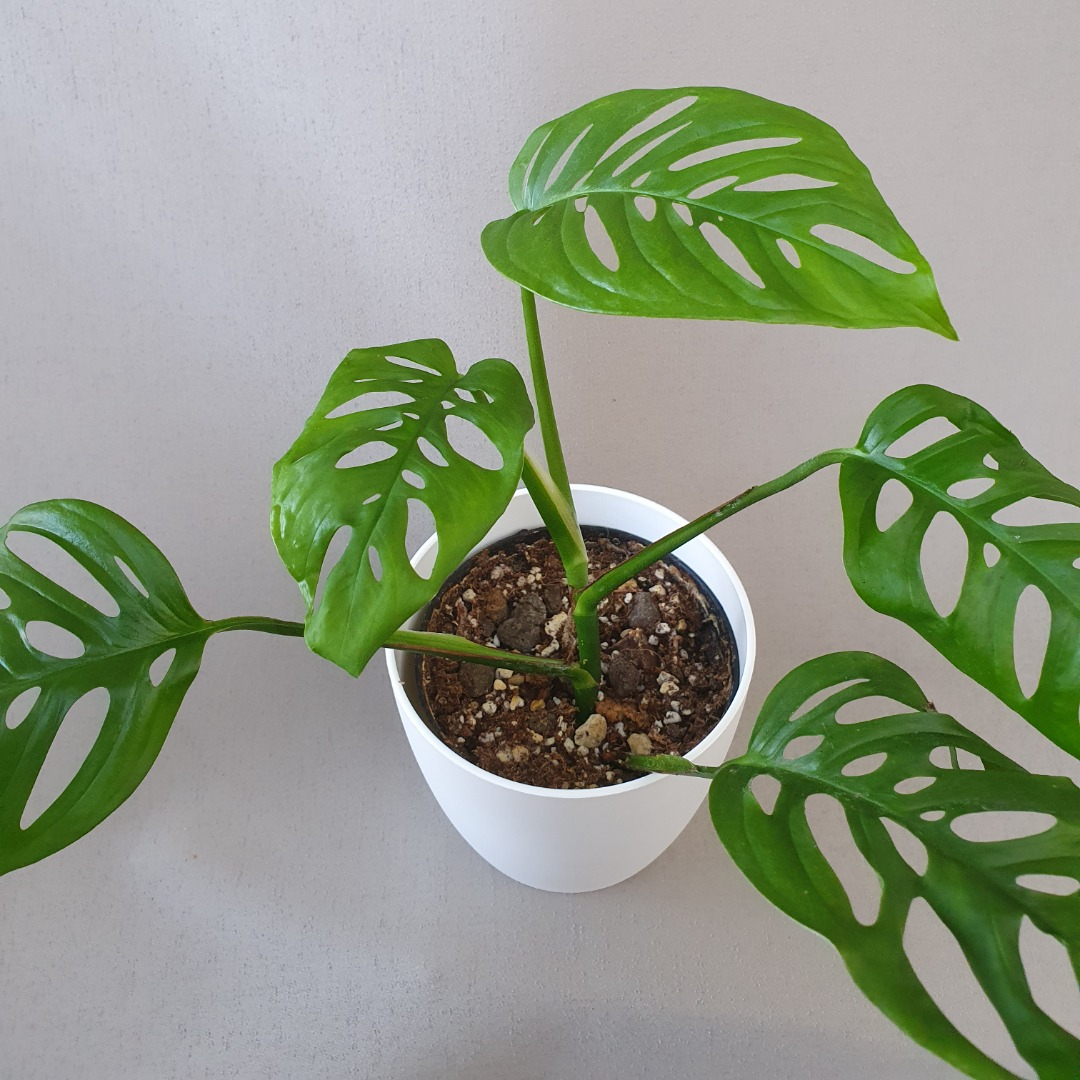
\includegraphics[width=.8\columnwidth]{img/pianta.jpg}

    5 foglie
  \end{figure}    
  \end{column}
  \begin{column}{0.4\textwidth}
    \begin{figure}
      
\includegraphics[width=.8\columnwidth]{img/caramelle.jpg}

      42 caramelle
    \end{figure} 
  \end{column}
\end{columns}}
\end{frame}


\begin{frame}
\frametitle{L'insieme $ \mathbb{N} $}
I numeri naturali corrispondono quindi all'insieme:
\[ \mathbb{N} = \{ 0, 1, 2, 3, 4, 5, \ldots \}\]\pause

\begin{figure}
  \begin{tikzpicture}
    \draw[thick, purple] (0,0) ellipse (3cm and 1.5cm);
    \node[purple] at (2,.4) {$ \mathbb{N} $};
    \node[below,purple] at (2,.4) {naturali};
    \node[] at (-2,0) {$ 2 $};
    \node[] at (0,1) {$ 10 $};
    \node[] at (1,-1) {$ 135 $};
    \node[] at (-.5,-1) {$ 0 $};
    \node[] at (0,0) {$ \ldots $};
\end{tikzpicture}
\end{figure}\pause

~

Attenzione: lo zero è un numero naturale!
\end{frame}

\begin{frame}
\frametitle{Visualizzazione dei naturali}
I numeri naturali possono essere visualizzati/immaginati come punti su una \alert{semiretta}.

~

\begin{figure}
  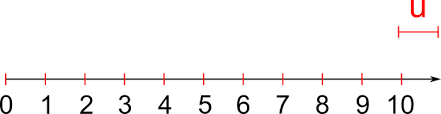
\includegraphics[width=.8\columnwidth]{img/naturali.png}
\end{figure}\pause

~

Immaginare i numeri (non solo i naturali) come punti sulla retta è fondamentale per capirli per davvero!
\end{frame}


\begin{frame}
\frametitle{Precedente e successivo}
\begin{figure}
  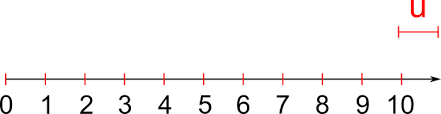
\includegraphics[width=.6\columnwidth]{img/naturali.png}
\end{figure}

~

Tutti i naturali, tranne lo zero, hanno un:
\begin{itemize}
  \item \alert{precedente}, cioè il numero immediatamente a sinistra sulla linea dei naturali;\pause
  \item \alert{successivo/conseguente}, cioè il numero immediatamente a destra sulla linea dei naturali;\pause
\end{itemize}

~

Lo zero ha solo il successivo, non ha il precedente.
\end{frame}


\begin{frame}
\frametitle{Confronto tra naturali}
L'insieme dei naturali è \alert{ordinato}, cioè alcuni numeri vengono prima (sono più piccoli) e altri vengono dopo (sono più grandi).\pause

~

\alert{Confrontare due naturali} significa stabilire se sono uguali e, se non lo sono, quale dei due è il più grande.\pause

~

I simboli utilizzati sono: 
\begin{itemize}
  \item $ = $ (uguale a);
  \item $ < $ (minore di);
  \item $ > $ (maggiore di).
\end{itemize}  
\end{frame}


\begin{frame}
\frametitle{Esempi}
\begin{figure}
  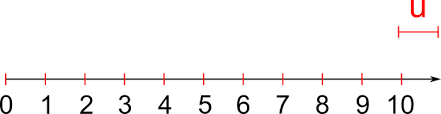
\includegraphics[width=.6\columnwidth]{img/naturali.png}
\end{figure}

\[ 5 = 5 \]\pause
\[ 5 < 7 \]\pause
\[ 5 > 4 \]\pause
\end{frame}

\section{Operazioni}

\begin{frame}
\frametitle{Somma o addizione}
La somma (simbolo $ + $) si esegue tra due numeri, partendo dal primo e contando verso destra tante unità quante sono nel secondo numero.

~
\begin{figure}
  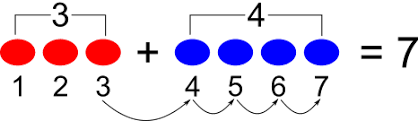
\includegraphics[width=.8\columnwidth]{img/somma.png}
\end{figure}

~

Per svolgere facilmente le somme, è sempre comodo \alert{visualizzarle}.
\end{frame}

\begin{frame}
\frametitle{Terminologia}
È utile imparare anche i termini corretti per indicare ciò di cui stiamo parlando:

~

\begin{figure}
  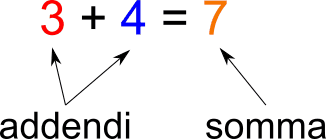
\includegraphics[width=.5\columnwidth]{img/somma2.png}
\end{figure}

~

Addendo significa ``cosa da sommare''.
\end{frame}

\begin{frame}
\frametitle{Proprietà della somma}
L'addizione è:
\begin{itemize}
  \item \alert{commutativa}, invertendo l'ordine degli addendi la somma non cambia:\[3+7=7+3\]\pause
  \item \alert{associativa}, la somma di tre o più addendi non cambia se al posto di alcuni di essi si sostituisce la loro somma:\[(4+7)+3=4+(7+3)\]\pause
  \item \alert{dissociativa}, la somma non cambia se un addendo viene sostituito con due addendi la cui somma è uguale a quello sostituito:\[7+ 13 = 7+ (3+10)\]
\end{itemize}
\end{frame}

\begin{frame}
\frametitle{Differenza o sottrazione}
La differenza (simbolo $ - $) si esegue tra due numeri, partendo dal primo e contando verso sinistra tante unità quante sono nel secondo numero.

~

\begin{figure}
  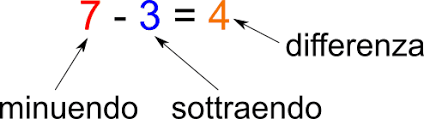
\includegraphics[width=.4\columnwidth]{img/differenza2.png}

  ~

  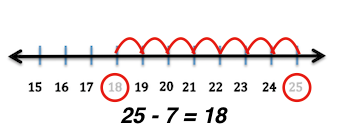
\includegraphics[width=.6\columnwidth]{img/differenza.png}
\end{figure}
\end{frame}

\begin{frame}
\frametitle{Un problema}
Se il minuendo è più piccolo del sottraendo, come in:\[7-12\]la differenza non può essere calcolata restando nell'insieme dei numeri naturali.

~

Vedremo che, per svolgere operazioni di questo tipo, è necessario un insieme di numeri diverso, l'insieme dei numeri interi $ \mathbb{Z} $.
\end{frame}


\begin{frame}
\frametitle{Prodotto o moltiplicazione}
Il prodotto (simbolo $ \times $ oppure $ \cdot $) si esegue tra due numeri, sommando il primo a sé stesso tante volte quante sono le unità del secondo numero.

~

\begin{figure}
  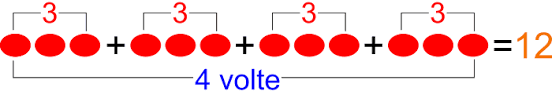
\includegraphics[width=.8\columnwidth]{img/prodotto2.png}

  ~

  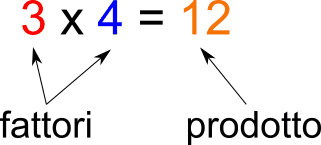
\includegraphics[width=.3\columnwidth]{img/prodotto.png}
\end{figure}\pause

Attenzione: il prodotto è commutativo, associativo e dissociativo!
\end{frame}


\begin{frame}
\frametitle{Proprietà distributiva}
Il prodotto ha un'altra utile proprietà, è distributivo rispetto alla somma e alla differenza. 

~

Ad esempio:

~

\[ 5 \cdot (\textcolor{blue}{3}\textcolor{orange}{+}\textcolor{red}{6}) = (5 \cdot \textcolor{blue}{3}) \textcolor{orange}{+} (5 \cdot \textcolor{red}{6})\]\pause

~

\[ 5 \cdot (\textcolor{blue}{7}\textcolor{orange}{-}\textcolor{red}{4}) = (5 \cdot \textcolor{blue}{7}) \textcolor{orange}{-} (5 \cdot \textcolor{red}{4})\]
\end{frame}


\begin{frame}
\frametitle{Quoziente o divisione}
Il quoziente (simbolo $ : $) si esegue tra due numeri. Si raggruppano le unità del primo in tanti gruppi uguali quante sono le unità del secondo e si contano le unità di un singolo gruppo.

~

\begin{figure}
  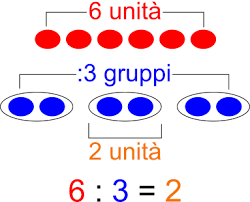
\includegraphics[width=.4\columnwidth]{img/divisione.png}
\end{figure}\pause

Perché non è possibile dividere per zero?
\end{frame}

\begin{frame}
\frametitle{Divisione con e senza resto}
Se la divisione può essere eseguita perfettamente (come $ 7:2 $), allora ci sono due possibilità:
\begin{itemize}
  \item si utilizza la divisione con il resto;\pause
  \item si utilizzano i numeri con la virgola (numeri decimali).
\end{itemize}
\end{frame}

\section{Potenze}

\begin{frame}
\frametitle{Elevamento a potenza}
L'elevamento a potenza utilizza due numeri, una \alert{base} e un \alert{esponente}. Si calcola moltiplicando la base per sé stessa tante volte quante indicate dall'esponente.

~

\begin{figure}
  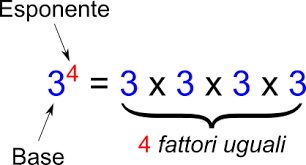
\includegraphics[width=.4\columnwidth]{img/potenza2.png}
\end{figure}\pause

~

Attenzione a non confondere l'elevamento a potenza con la moltiplicazione!
\end{frame}


\begin{frame}
\frametitle{Elevamenti particolari}
\[a^1 = a \]

\[ a^0 = 1\]
\end{frame}

\begin{frame}
\frametitle{Potenze di 10}
Molto utili e importanti sono le potenze di 10:
\[10^0 = 1\]\pause
\[10^1 = 10\]\pause
\[10^2 = 100\]\pause
\[10^3 = 1.000\]\pause
\[10^6 = 1.000.000\]\pause
\[10^9 = 1.000.000.000\]\pause
\end{frame}


\begin{frame}
\frametitle{Esercizi sulle potenze}
\begin{enumerate}
  \item Calcola il valore delle seguenti potenze:
  \begin{multicols}{2}
    \begin{itemize}
        \item $ 3^2 $
        \item $ 12^2 $
        \item $ 2^5 $
        \item $ 8^3 $
        \item $ 3^4 $
        \item $ 2^{10} $
    \end{itemize}
  \end{multicols}
  \item Trova il valore dell'esponente $ k $ in modo che siano vere le seguenti uguaglianze:
  \begin{multicols}{2}
    \begin{itemize}
        \item $ 3^k = 81 $
        \item $ 2^k = 256 $
        \item $ 5^k = 625 $
        \item $ 1765^k = 1765 $
    \end{itemize}
  \end{multicols}
  \item Disponi i seguenti numeri in ordine crescente:
  \[ 3^2\qquad 5^1\qquad 18\qquad 124\qquad 200^0\qquad 6^2\qquad 5^3 \]
\end{enumerate}
\end{frame}


\begin{frame}
\frametitle{Proprietà delle potenze}
Le proprietà delle potenze ci aiutano moltissimo a semplificare i calcoli che coinvolgono le potenze.\pause

~

\begin{itemize}
  \item Prodotto di potenze con la stessa base:
  \[a^{\textcolor{red}{m}} \cdot a^{\textcolor{red}{n}} = a^{\textcolor{red}{m+n}}\]
  Esempio:
  \[2^3 \cdot 2^7 = 2^{3+7} = 2^{10} \]
\end{itemize}
\end{frame}


\begin{frame}
\frametitle{Proprietà delle potenze}
\begin{itemize}
  \item Quoziente di potenze con la stessa base:
  \[a^{\textcolor{red}{m}} : a^{\textcolor{red}{n}} = a^{\textcolor{red}{m-n}}\]
  Esempio:
  \[2^7 : 2^5 = 2^{7-5} = 2^{2} \]\pause
  \item Potenza di potenza:\[(a^{\textcolor{red}{m}})^{\textcolor{red}{n}} = a^{\textcolor{red}{m\cdot n}}\]
  Esempio:
  \[(9^7)^2 = 9^{7\cdot 2} = 9^{14} \]
\end{itemize}
\end{frame}


\begin{frame}
\frametitle{Proprietà delle potenze}
\begin{itemize}
  \item Prodotto di potenze con lo stesso esponente:
  \[ {\textcolor{red}{a}}^n {\textcolor{red}{\cdot b}}^n = {\textcolor{red}{(a \cdot b)}}^n \]
  Esempio:
  \[2^7 \cdot 5^7 = (2 \cdot 5)^{7} = 10^{7} \]\pause
  \item Quoziente di potenze con lo stesso esponente:
  \[ {\textcolor{red}{a}}^n {\textcolor{red}{: b}}^n = {\textcolor{red}{(a : b)}}^n \]
  Esempio:
  \[14^8 : 7^8 = (14 : 7)^{8} = 2^{8} \]
\end{itemize}
\end{frame}


\begin{frame}
\frametitle{Esercizi sulle proprietà delle potenze}
\begin{enumerate}
  \item Calcola applicando le proprietà delle potenze:
  \begin{multicols}{2}
    \begin{itemize}
        \item $ 2^4 \cdot 2^6 : 2^{10} $
        
        ~

        \item $ \left[ (7^2)^3\right]^4 : \left[(7^3)^2\right]^0 $
        
        
        ~

        \item $ a^3 : a^2 $
        \item $ 3^4 \cdot 3^5 : 3^6 $
        
        
        ~

        \item $ \left[ (2^3 \cdot 3^3)^4 : 6^{10} \right]^2 : (2^2 \cdot 3^2)^2 $
        
        
        ~

        \item $ (a^7)^3 $
    \end{itemize}
  \end{multicols}
  \item Trova il valore di $ x $ in modo che siano vere le seguenti uguaglianze:
  \begin{multicols}{2}
    \begin{itemize}
        \item $ 3^{x+2} = 27 $
        \item $ 2^{4-x} = 2 $
    \end{itemize}
  \end{multicols}
\end{enumerate}
\end{frame}


\section{Espressioni}

\begin{frame}
\frametitle{Espressioni}
Una espressione matematica è una sequenza di calcoli, come ad esempio:

\[8+45:3^2+4\cdot 2-14\]
  
Come si esegue? In quale ordine si eseguono le operazioni?
\end{frame}


\begin{frame}
\frametitle{Espressioni senza parentesi}
Quando l'espressione è senza parentesi, le operazioni vanno eseguite in questo ordine (rimangono vere le proprietà che abbiamo visto):
\begin{enumerate}
  \item elevamento a potenza;
  \item moltiplicazioni e divisioni;
  \item somme e sottrazioni.
\end{enumerate}
\end{frame}


\begin{frame}
\frametitle{Esempio}

\[8+45:\textcolor{red}{3^2}+4\cdot 2-14 = \]\pause

~

\[= 8+\textcolor{red}{45:9}+\textcolor{red}{4\cdot 2}-14 = \]\pause

~

\[= \textcolor{red}{8+5+8-14} = 7 \]
\end{frame}


\begin{frame}
\frametitle{Espressioni con le parentesi}
In questo caso si \alert{ragiona a blocchi}, svolgendo prima di tutto le operazioni nelle parentesi più interne.\pause

~

Prova a calcolare:
\[ 42 : \{ 105 : [(5 \cdot 2^2 + 7) : 3^2 + (7^2 : 7 + 3) : 5] \} \]
\end{frame}



\begin{frame}
\frametitle{Esercizi sulle espressioni (1)}
\begin{enumerate}
  \item Traduci in espressioni aritmetiche le seguenti frasi e calcola poi il loro valore.
  \vspace*{.15cm}
  \begin{itemize}
    \item Aggiungi a 72 il prodotto tra 7 e 8.
    \vspace*{.15cm}
    \item Moltiplica la differenza di 17 e 8 per la somma di 2 e 3.
    \vspace*{.15cm}
    \item Sottrai al prodotto di 7 e 4 il quoziente di 36 e 12.
    \vspace*{.15cm}
    \item Moltiplica la somma di 5 e 8 per 2 e sottrai al risultato 10.
  \end{itemize}
  \vspace*{.25cm}
  \item Calcola il valore delle seguenti espressioni:
  \vspace*{.15cm}
  \begin{itemize}
    \item $  1 + [(15 : 3) \cdot 7+ (10 \cdot 2): 4] : (2\cdot4) - [(2\cdot5): 2 - 2] $
    \vspace*{.15cm}
    \item $ \{[(6\cdot 4 - 18) + 5\cdot (12-9)]: (7\cdot 2-11) -3+10\} : 7 $
    \vspace*{.15cm}
    \item $ [5 \cdot (3 \cdot 8-5 \cdot 4) - 7 ] \{4 \cdot (28: 7+4): [(6 \cdot 5): 15] -2 \cdot 8\} $
  \end{itemize}
\end{enumerate}
\end{frame}


\begin{frame}
\frametitle{Esercizi sulle espressioni (2)}
\begin{enumerate}\setcounter{enumi}{2}
  \item Calcola il valore delle seguenti espressioni:
  \vspace*{.15cm}
  \begin{itemize}
    \item $  [(3^6 : 3^4) - 2^3] \cdot [(5^3 \cdot 5^4) : (5^2 \cdot 5^3)] : (2^2 + 1) $
    
    \hspace{\fill}[$ 5 $]
    \vspace*{.25cm}
    \item $  \{[(3^{10} : 3^6)^2 \cdot (3^8:3^3)] : 3^{12}\} + 1^7 + (2^2 \cdot 3 - 11) $
    
    \hspace{\fill}[$ 5 $]
    \vspace*{.25cm}
    \item $  [(6^3\cdot 2^3 : 4^3) : (10^4 : 5^4 - 7)\cdot 3^4]^2 : (3^3\cdot 3^2)^2 $
    
    \hspace{\fill}[$ 1 $]
    \vspace*{.25cm}
    \item $ 2^2 + \{[(3 \cdot 2^2 + 2) \cdot 2 - 6 \cdot 2 + (2 \cdot 6 + 1^5 \cdot 7)] : 5 + 7\} : 14 +4 $
    
    \hspace{\fill}[$ 9 $]
  \end{itemize}
\end{enumerate}
\end{frame}


\section{Numeri interi}


\begin{frame}
\frametitle{Un nuovo insieme di numeri}
I numeri interi o relativi, sono tutti numeri interi (senza virgola) e sono caratterizzati da un segno negativo, nullo o positivo:
\[ \mathbb{Z} = \{ \ldots, -5, -4, -3, -2, -1, 0, +1, +2, +3, +4, +5, \ldots \}\]\pause
Il nuovo insieme \alert{include} il precedente insieme $ \mathbb{N} $.

~

\visible<2->{\begin{figure}
  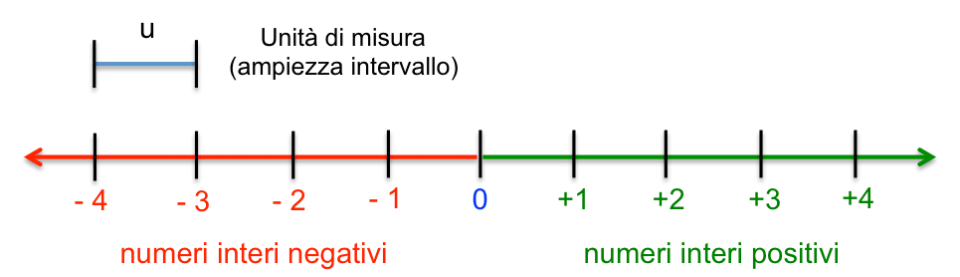
\includegraphics[width=.8\columnwidth]{img/rettarelativi.png}
\end{figure}}\pause
Per comodità, a volte il segno + viene omesso, e quindi scrivere $ +6 $ oppure semplicemente $ 6 $ è la stessa cosa.
\end{frame}



\begin{frame}
\frametitle{Utilizzi dei negativi}
I numeri negativi permettono di svolgere operazioni che erano impossibili nell'insieme $ \mathbb{N} $ dei naturali, ad esempio:
\[18- 20 \]\pause
Ora possiamo dire che il risultato di $ 18-20 $ è $ -2 $.\pause

~

I numeri negativi vengono utilizzati anche nella vita reale:
\visible<3->{\begin{figure}
  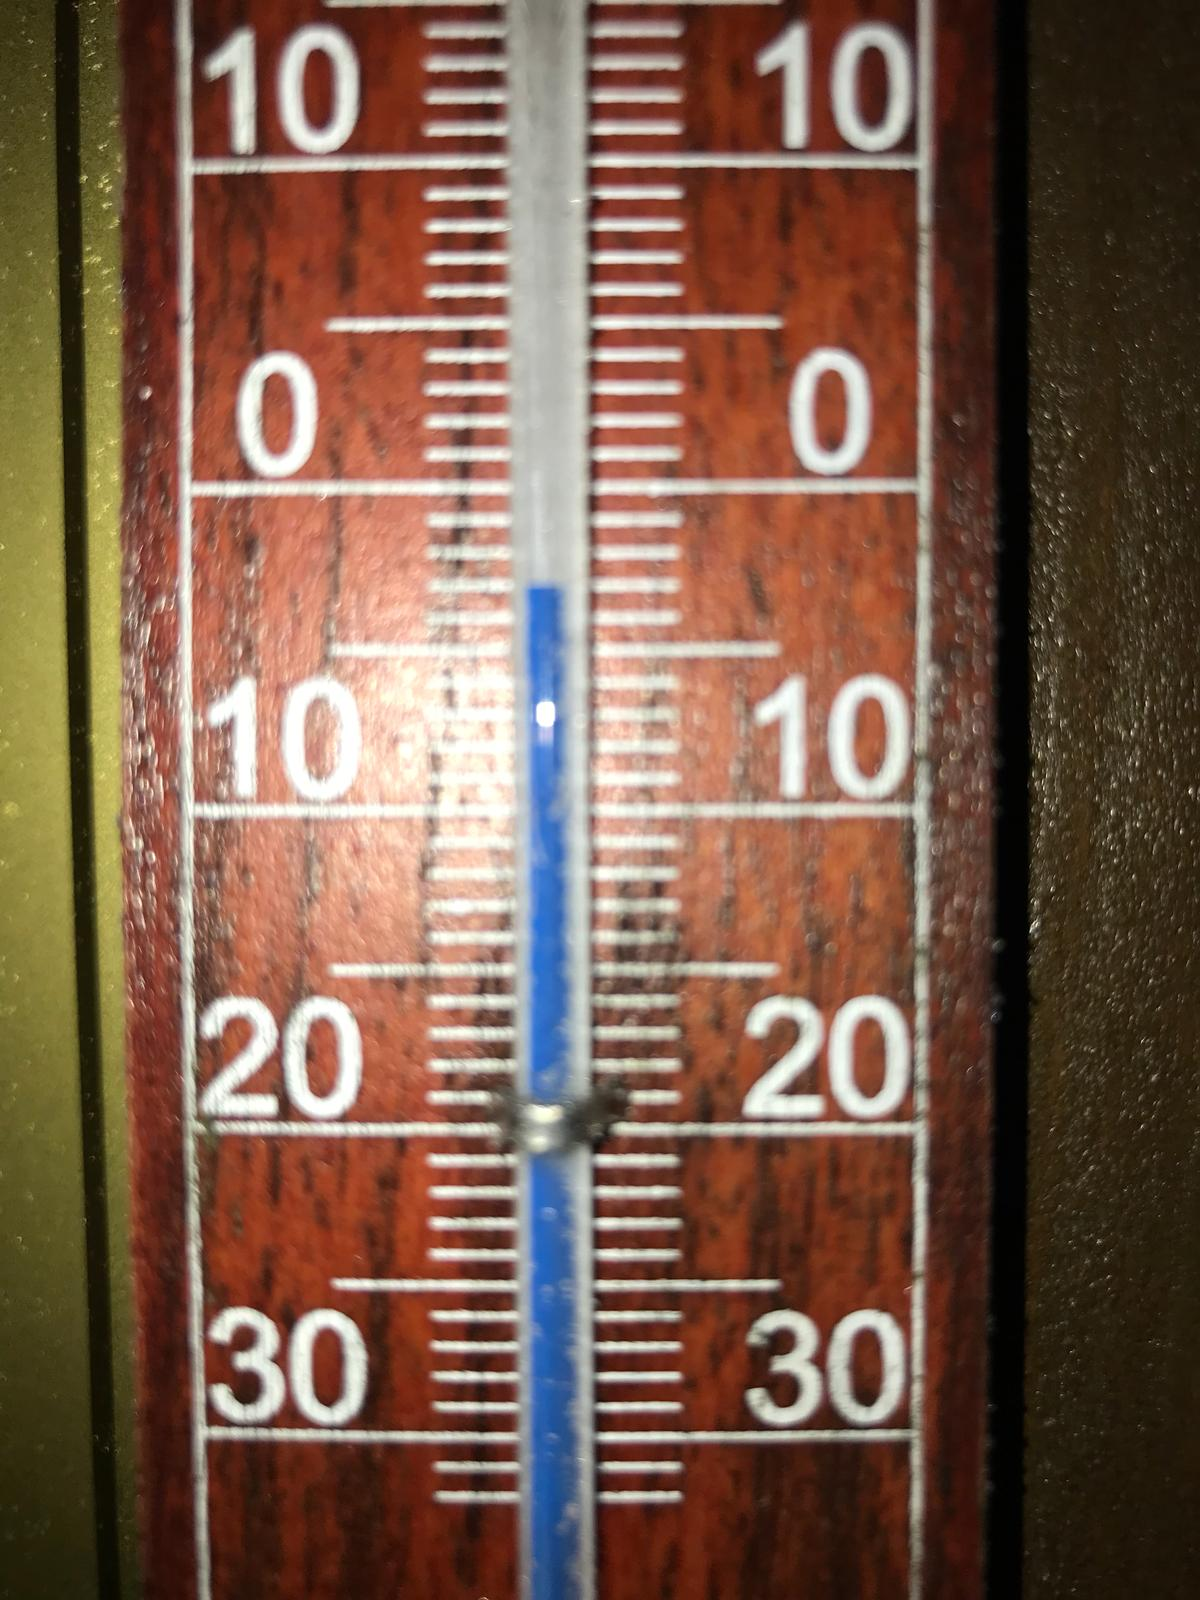
\includegraphics[width=.25\columnwidth]{img/termometro.jpg}
\end{figure}}
\end{frame}


\begin{frame}
\frametitle{Valore assoluto}
Per capire il concetto di valore assoluto è importante \alert{visualizzare} i numeri interi:
\begin{figure}
  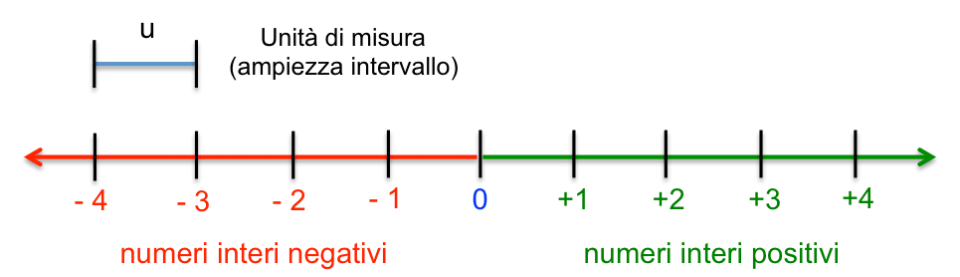
\includegraphics[width=.8\columnwidth]{img/rettarelativi.png}
\end{figure}\pause
Il valore assoluto di un numero si indica con \alert{due sbarrette intorno ad un numero}, come:
\[|-7|\]
\end{frame}

\begin{frame}
\frametitle{Valore assoluto come distanza}
Il valore assoluto di un numero corrisponde alla \alert{distanza del numero dallo 0} sulla retta dei numeri.
\begin{figure}
  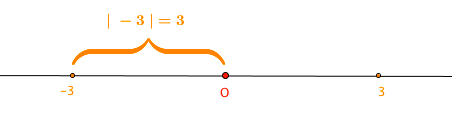
\includegraphics[width=.8\columnwidth]{img/modulodistanza.png}
\end{figure}
Quindi:
\[|-3| = |+3| = 3\]\pause

Quali due numeri interi hanno valore assoluto pari a 14?
\end{frame}

\begin{frame}
\frametitle{Terminologia}
Vediamo alcune utili definizioni:
\begin{itemize}
  \item \alert{numeri concordi}, se hanno lo stesso segno, come:
  \begin{center}
    $ -7 $ e $ -100 $
  \end{center}\pause
  \item \alert{numeri discordi}, se hanno segno diverso, come:
  \begin{center}
    $ -12 $ e $ +4 $
  \end{center}\pause
  \item \alert{numeri opposti}, se hanno lo stesso valore assoluto e segno diverso, come:
  \begin{center}
    $ -8 $ e $ +8 $
  \end{center}
\end{itemize}
\end{frame}


\begin{frame}
\frametitle{Confronto tra numeri interi}
Il confronto tra numeri interi, indicato con $ = $, $ > $ e $ < $, avviene come per i numeri naturali.\pause

~

È sempre bene \alert{visualizzare i numeri interi} per poterli confrontare bene. Numeri che sono più a destra sono più grandi, numeri che sono più a sinistra sono più piccoli.\pause

\[ -3 < +9 \]\pause
\[ -23 < -1 \]\pause
\[ +13 > +2\]\pause
\[ +6 > -300 \]
\end{frame}

\begin{frame}
\frametitle{Somme e sottrazioni}
\alert{La somma e la sottrazione si svolgono come per i numeri naturali}, spostandosi a destra o sinistra sulla retta dei numeri:

\begin{figure}
  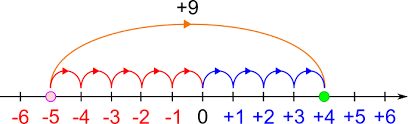
\includegraphics[width=.8\columnwidth]{img/sommainteri.png}

  ~

  $ -5 + 9 = +4 $
\end{figure}\pause

Non ci sono regole ``strane'' da applicare!
\end{frame}


\begin{frame}
\frametitle{La regola dei segni}
Per svolgere moltiplicazioni e divisioni dobbiamo invece studiare la regola dei segni:

~

\begin{block}{Regola dei segni (1)}
  Il prodotto/quoziente di numeri con lo \alert{stesso segno} è un numero \alert{positivo}.

  \[ (+5)\cdot(+2) = +10 \qquad\qquad\qquad (-3):(-1) = +3\]\pause

  Il prodotto/quoziente di numeri con \alert{segno diverso} è un numero \alert{negativo}. 

  \[ (+4)\cdot(-3) = -12 \qquad\qquad\qquad (-9):(+3) = -3\]
\end{block}
\end{frame}

\begin{frame}
\frametitle{Regola dei segni per le potenze} 
\begin{block}{Regola dei segni (2)}
  Le \alert{potenze pari} di qualsiasi numero \alert{sono positive}.

  \[ (+2)^4 = +16 \qquad\qquad\qquad (-2)^4 = +16 \]\pause

  Le \alert{potenze dispari} invece \alert{mantengono il segno della base}.

  \[ (+4)^3 = +64 \qquad\qquad\qquad (-4)^3 = -64 \]
\end{block}\pause

Riesci a spiegare perché?
\end{frame}


\begin{frame}
\frametitle{Esercizi su somma e differenza di numeri interi}
\begin{enumerate}\setcounter{enumi}{0}
  \item Completa la tabella:
\end{enumerate}
\begin{figure}
  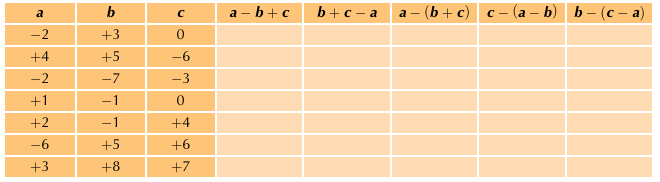
\includegraphics[width=\columnwidth]{img/eseinteri.png}
\end{figure}
\begin{enumerate}\setcounter{enumi}{1}
  \item Inserisci al posto dei puntini il numero mancante:
  \begin{multicols}{2}
    \begin{itemize}
      \item $ (+14) + (\ldots) = -8 $
      
      ~
      \item $ (-12) + (\ldots) = +5 $
      \item $ (\ldots) - (-4) = -6 $
      
      ~
      \item $ (+3) - (\ldots) = +8 $
    \end{itemize}
  \end{multicols}
\end{enumerate}
\end{frame}



\begin{frame}
\frametitle{Esercizi su somma e differenza di numeri interi}
\begin{enumerate}\setcounter{enumi}{0}
  \item Completa la tabella:
\end{enumerate}
\begin{figure}
  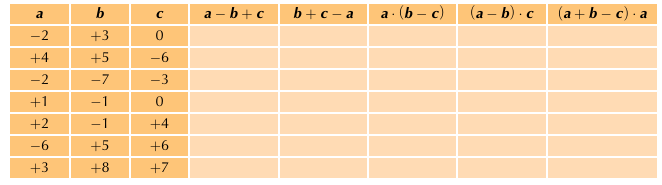
\includegraphics[width=\columnwidth]{img/eseinteri1.png}
\end{figure}
\begin{enumerate}\setcounter{enumi}{1}
  \item Inserisci al posto dei puntini il numero mancante:
  \begin{multicols}{2}
    \begin{itemize}
      \item $ (-9) \cdot (\ldots) = +108 $
      
      ~
      \item $ (+3) \cdot (\ldots) = -48 $
      \item $ (\ldots) \cdot (-8) = -104 $
      
      ~
      \item $ (-32) : (\ldots) = +4 $
    \end{itemize}
  \end{multicols}
\end{enumerate}
\end{frame}


\begin{frame}
\frametitle{Espressioni coi numeri interi}
\begin{enumerate}
  \item Calcola il valore delle seguenti espressioni:
  \vspace*{.15cm}
  \begin{itemize}
    \item $  \{-14+3 \cdot [9+ 2 \cdot (-2) - 3 \cdot (17 + 2 - 15)]\} \cdot (-1) $
    
    \hspace{\fill}[$ +35 $]%184
    \vspace*{.25cm}
    \item $ [25 - (-13 +12)] : 13 + [3 + 2(-12 - 4) : (+5 + 3) - 1] $
    
    \hspace{\fill}[$ 0 $]%185
    \vspace*{.25cm}
    \item $  \{[(-8)^2]^5\}^3 : \{[(-8)^3]^2\}^5 $
    
    \hspace{\fill}[$ 1 $]%203
    \vspace*{.25cm}
    \item $ [(-5) ^2\cdot (-5)^3 : (-5)^4]^2 - (8 - 2^2 - 3^2) \cdot  (5^6 : 5^4 - 30) $
    
    \hspace{\fill}[$ 0 $]%212
  \end{itemize}
\end{enumerate}
\end{frame}

\begin{frame}
\frametitle{Un'espressione speciale}
\footnotesize{ $ \left\{ -7 + \left[ - (-4 + 13^0) + (-6+2-1)^2 \cdot (5-7)^2 : (8-2-6) \right]^2 \right\} : \left[ (-3)^2 \right]^2 $}\pause%222

  ~

  ~

  ~
\normalsize
  Perché questa espressione è \alert{impossibile}?
\end{frame}



\section{Numeri decimali}


\begin{frame}
\frametitle{Cosa sono i numeri decimali?}
I numeri decimali sono numeri formati da \alert{due parti}:
\begin{itemize}
  \item una \alert{parte intera}, prima della virgola;\pause
  \item una \alert{parte decimale}, dopo la virgola.\pause
\end{itemize}
Sono numeri che utilizziamo tutti i giorni, ad esempio per i prezzi o i pesi dei prodotti.

\begin{figure}
  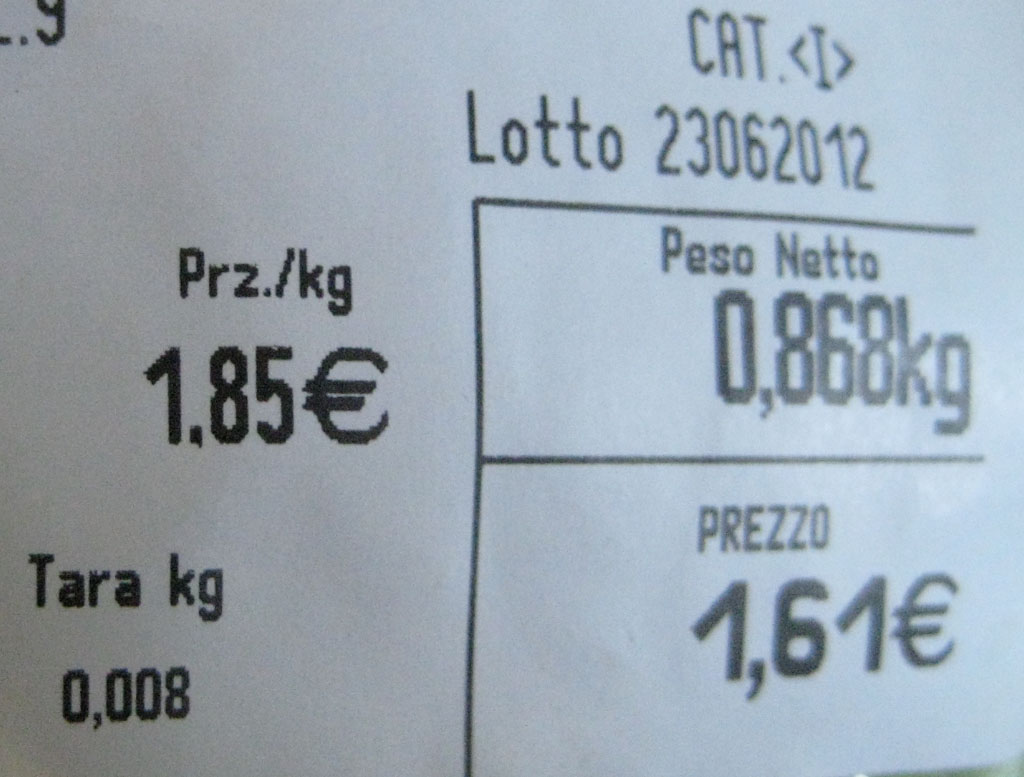
\includegraphics[width=.4\columnwidth]{img/scontrino.jpg}
\end{figure}
\end{frame}


\begin{frame}
\frametitle{Nomi delle cifre decimali}
\begin{table}[]\def\arraystretch{1.5}
  \begin{tabular}{|r|c|c|c|}\hline
  \textbf{Nome della cifra} & \textbf{Posizione} & \textbf{Valore} & \textbf{Simbolo} \\\hline
  decimi                    & 1                  & 0,1             & d                \\\hline
  centesimi                 & 2                  & 0,01            & c                \\\hline
  millesimi                 & 3                  & 0,001           & m                \\\hline
  \end{tabular}
\end{table}\pause

~

Esempio:
\[ 4,745 \]
4 unità, 7 decimi, 4 centesimi e 5 millesimi
\end{frame}



\begin{frame}
\frametitle{Confronto tra decimali}
Quando confrontiamo due decimali, attenzione a fare il confronto \alert{cifra per cifra}: confrontare le unità con le unità, i decimi con i decimi, ecc.\pause

~

Esempio:
\[ 7,099 < 7,12 \]
La prima cifra per cui differiscono sono i decimi, ed è quella da guardare per ordinare i numeri.
\end{frame}


\begin{frame}
\frametitle{Rapresentazione dei decimali}
Come tutti gli altri numeri, anche i decimali si possono \alert{visualizzare su una retta orientata}:

\begin{figure}
  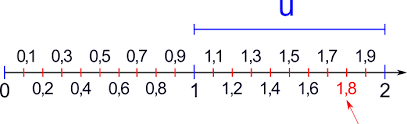
\includegraphics[width=.8\columnwidth]{img/rettadecimali.png}
\end{figure}
\end{frame}




\begin{frame}
\frametitle{Esercizi sull'ordinamento dei decimali}
\begin{enumerate}
  \item Disponi in ordine crescente i seguenti numeri decimali:
    \[ 1,8\qquad0,3\qquad1,5\qquad6,9\qquad5,3\qquad1,799\qquad1,485\qquad0,305 \]
  \item Completa le seguenti frasi:
  
  ~
    \begin{itemize}
        \item 1000 millesimi formano \ldots unità.
        
        ~
        \item 2000 centesimi formano \ldots unità.
        
        ~
        \item 200 decimi formano \ldots unità.
        
        ~
        \item 4000 decimi formano \ldots unità.
    \end{itemize}
\end{enumerate}
\end{frame}



\begin{frame}
\frametitle{Operazioni coi decimali}
Le operazioni coi decimali seguono le stesse regole di tutti gli altri numeri.\pause

~

È molto comodo visualizzare somme e sottrazioni \alert{in colonna}, per non confondersi con le cifre decimali.

~

Per eseguire 5,15 + 2,743 facciamo:
\begin{table}[]\def\arraystretch{1.2}
  \begin{tabular}{llllll}
  5 & , & 1 & 5 &   & + \\
  2 & , & 7 & 4 & 3 & = \\\hline
  7 & , & 8 & 9 & 3 &   \\
  \end{tabular}
  \end{table}

\end{frame}



\begin{frame}
\frametitle{Approssimare}
A volte, nei nostri calcoli con la calcolatrice, otteniamo numeri ``scomodi'', come:
\[5,1814894\]

~

Spesso non ci interessano più di \alert{due o tre cifre decimali}, e vogliamo quindi ``tagliare'' il numero, cioè \alert{approssimarlo}.\pause

~

5,18 è una approssimazione accettabile del numero precedente.
\end{frame}



\begin{frame}
\frametitle{Regole per approssimare}
Prima di tutto dobbiamo \alert{decidere a quale cifra approssimare}: ai decimi (una cifra), ai centesimi (due cifre) o ai millesimi (tre cifre).\pause

~

Dobbiamo poi guardare \alert{la cifra successiva all'ultima che vogliamo scrivere}:\pause

~
\begin{itemize}
  \item se la cifra successiva è 0, 1, 2, 3 o 4, approssimiamo per \alert{difetto}, eliminando la parte che non vogliamo;\pause
  
  ~
  \item se la cifra successiva è 5, 6, 7, 8 o 9, approssimiamo per \alert{eccesso}, aumentando di 1 l'ultima cifra che scriviamo.
\end{itemize}
\end{frame}



\begin{frame}
\frametitle{Esempi}
\[\alert<2->{7,2}\alert<3->{7}\alert<4->{3}5\]\pause

Approssimazione ai decimi: 7,3.\pause

~

Approssimazione ai centesimi: 7,27.\pause

~

Approssimazione ai millesimi: 7,274.
\end{frame}




\begin{frame}
\frametitle{Esercizi sull'approssimazione dei decimali}
\begin{enumerate}
  \item Approssima i seguenti numeri a una cifra decimale:
    \[ 1,83\qquad0,35\qquad1,485\qquad0,3058178 \]
  \item Approssima i seguenti numeri a due cifre decimali:
    \[ 6,099\qquad4,0673\qquad9,005\qquad3,2324 \]

\end{enumerate}
\end{frame}



\begin{frame}
\frametitle{E le frazioni?}
I numeri decimali, sia positivi sia negativi, possono essere anche espressi sotto forma di \alert{frazioni}, che vanno a costituire l'insieme $ \mathbb{Q} $ dei \alert{numeri razionali}.\pause

~

Ad esempio:
\begin{center}
  $ 7,7 = 77 : 10 = \dfrac{77}{10} $\pause
  
  ~

  ~

  $ -2,3 = -23 : 10 = -\dfrac{23}{10} $
\end{center}\pause

Le frazioni sono solo un modo più comodo di scrivere delle divisioni!
\end{frame}


\begin{frame}
\frametitle{Insiemi numerici}

\begin{figure}
  \begin{tikzpicture}
    \draw[thick, purple] (0,0) ellipse (3cm and 1.5cm);
    \node[purple] at (2,.4) {$ \mathbb{N} $};
    \node[below,purple] at (2,.4) {naturali};
    \node[] at (-2,0) {$ 2 $};
    \node[] at (0,1) {$ 10 $};
    \node[] at (1,-1) {$ 135 $};
    \draw[thick, blue] (.6,0) ellipse (4cm and 2.5cm);
    \node[blue] at (3.8,.4) {$ \mathbb{Z} $};
    \node[below,blue] at (3.8,.4) {interi};
    \node[] at (2.5,1.3) {$ -6 $};
    \node[] at (1,-1.8) {$ -1 $};
    \node[] at (1,1.8) {$ 100 $};
    \draw[thick, red] (1.2,0) ellipse (5cm and 3.5cm);
    \node[red] at (5.4,.4) {$ \mathbb{Q} $};
    \node[below,red] at (5.4,.4) {razionali};
    \node[] at (4.5,1.7) {$ \dfrac{2}{3} $};
    \node[] at (4.5,-1.7) {$ -\dfrac{23}{10} $};
    \node[] at (3,-2.7) {$ \dfrac{16}{7} $};
\end{tikzpicture}
\end{figure}
\end{frame}

\end{document}
